\documentclass[11pt]{article}

\usepackage{amsmath}
\usepackage{graphicx}
\usepackage[left=2cm, right=2cm, bottom=3cm, top=3cm]{geometry}

\graphicspath{ {../../Images} }
\title{Results of the Bayesian model (Draft)}
\author{Alexandre Y. Péré}
\date{\today}

\begin{document}
    \maketitle
    
    \section{Overall approach}
    In this document we present the current results of the Bayesian approach to the cancer immunotherapy project. 

    It must first be noted that in addition to the model presented in the ``Bayesian Analysis Approach'' document (which will be referred to as the mutimodal model), we introduce a new yet very similar model, called the unimodal model. The only difference is that in the unimodal model, all the priors are unimodal normal distributions. The reason for this will be discussed in Section 2. 

    Before  using the models with real experimental data, we first perform a validation test to check if they are reliable and working as expected. This is the topic of Section 2 and 3.

    The current analysis considers that the parameters of interest $k_6$, $d_1$ and $s_2$, following Christian's sensitivity analysis. However, this set of parameters of interest might change in the future, once the positive feedback loop will be integrated in the model. If this happens, we will re-run all the tests and inferences with this new set of parameters. However, we think that the results presented in this document are still relevant, since they concern the whole model.


    \section{Validation of the unimodal hierarchical model}
    This model is a Bayesian hierarchical model similar to the one presented in the ``Bayesian Analysis Proposal" document, the only difference being that priors are unimodal normal distributions (and not Gaussian mixture models). This results in less hyperparameters (two for each individual parameters: a mean $\mu$ and a standard deviation $\sigma$). The purpose of this model is twofold. As the parameter space is smaller, it is faster to perform inferences, check the model and potentially improve it, with most improvements being transferrable to the multimodal model. It can also act as a comparison point with the multimodal model (once it is validated).
    
        \subsection{Methods}
    Posterior distributions were sampled with the default No U-Turn Sampler implemented in Julia (1000 samples per chain, 4 chains in parallel, unspecified acceptance rate). The validation dataset was composed of two time series, corresponding to the simulated tumour evolution for two mice.  These time series were simulated using parameters sampled from artifical population distributions (I will add them in the appendix soon). To better emulate the experimental data, only 9 data points were picked from these simulations, corresponding to days of data collection from the experiments (the other data points were discarded).\\
    The model relies on logtransformation of the parameters, hence in the following graphs the values are actually the log of the parameters.

        \subsection{Estimation of individual parameters}
    First we demonstrate that the unimodal model is able to estimate, for each time series, the set of parameters that was used to generate it.

    Fig. \ref{fig:ind_params} shows the posterior distributions of each parameter of mouse~1. The vertical lines indicate the true value that was used to generate its time series. As we can see, the estimation for $s_2$ are very accurate, while there is some offset for both $k_6$ and $d_1$. This might be due to the MCMC chains being too short, to verify this we will run longer chains. We also suspect that the model in too reliant on the priors, which can induce some noticable offset if the priors are not exactly centered on the true value (which is often the case). We are currently trying to improve this behaviour. 

    \begin{figure}[!h]
        \centering
        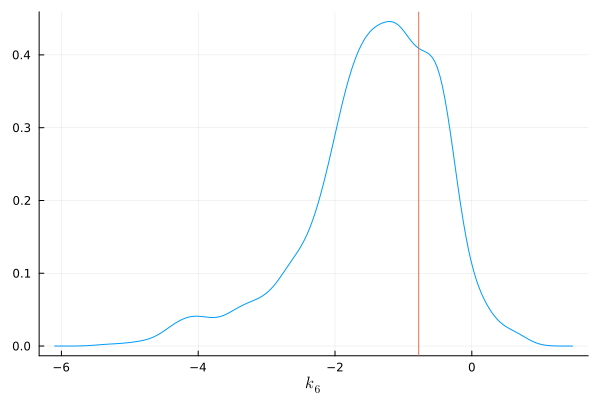
\includegraphics[scale=0.4]{k6_1.png}
        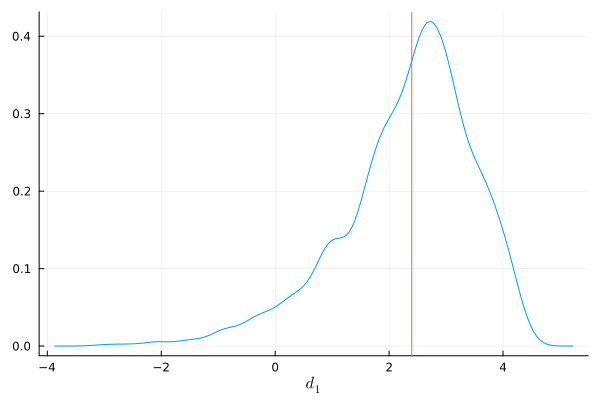
\includegraphics[scale=0.4]{d1_1.png}
        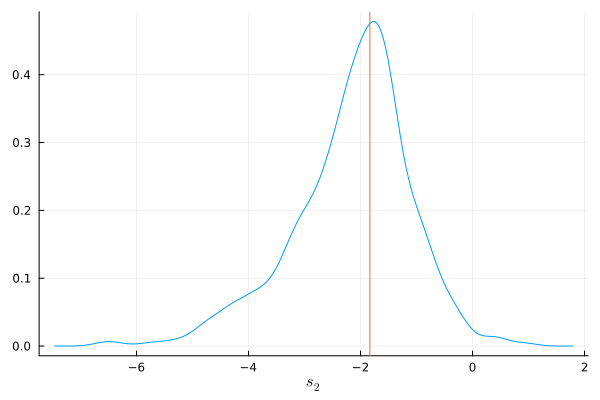
\includegraphics[scale=0.4]{s2_1.png}
        \caption{Posterior distribution of the parameters of interest for mouse 1}
        \label{fig:ind_params}
    \end{figure}
    
    Fig. \ref{fig:simul} was constructed by sampling 300 set of parameters from the posterior distributions and simulating the system for each set. The solid blue line is the median time series, while the shaded area represents the 70\% density predictions. The pink dots represent the validation data points. It can be observed that there is a non-negligible, systematic difference between the median curve and the ``true" one. This is still under investigation, but it is likely that this problem is linked to the offset highlighted in the previous paragraph. 

    \begin{figure}[!h]
        \centering
        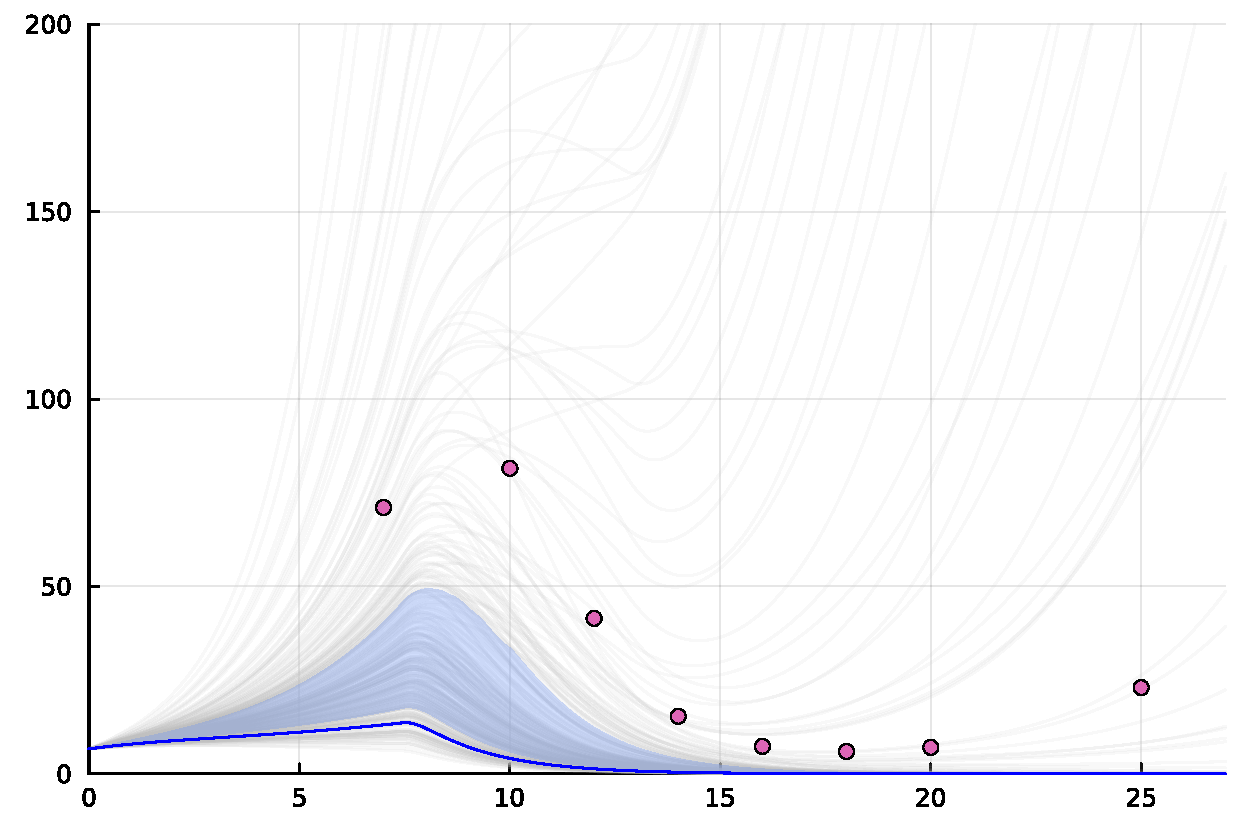
\includegraphics[scale=0.4]{simul.pdf}
        \caption{Simulation of the tumour evolution using estimated parameters}
        \label{fig:simul}
    \end{figure}
    
    
        \subsection{Estimation of population distributions}
    In this subsection we show that the model can fulfill its main goal, which is to estimate the population distributions for the parameters of interest (namely $k_6$, $d_1$, $s_2$). 

    Fig. \ref{fig:pop_d1} shows these population distributions. The orange curves represent the ``true" distributions, ie those from which the individual parameters were sampled to generate the validation dataset. The blue curves are the model's estimation of these population distributions, which were reconstructed from the posterior distributions of the hyperparameters. 
    
    As we can see, the estimation are relatively close to the true distributions. The slight offset is most likely linked to the problem highlighted in the previous section. However, in this case it is also likely that the estimation quality will improve when using a larger pool of mice.

    \begin{figure}[!h]
        \centering
        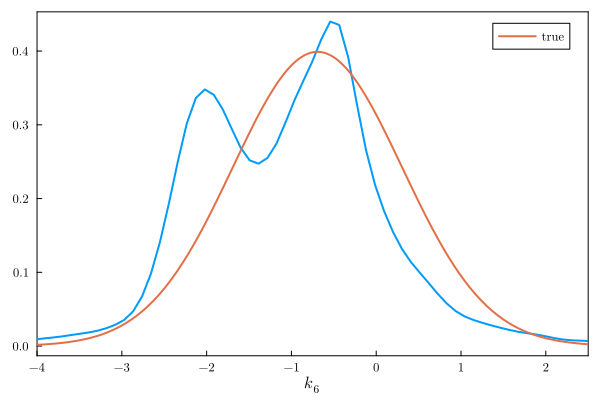
\includegraphics[scale=0.4]{k6_popu.png}
        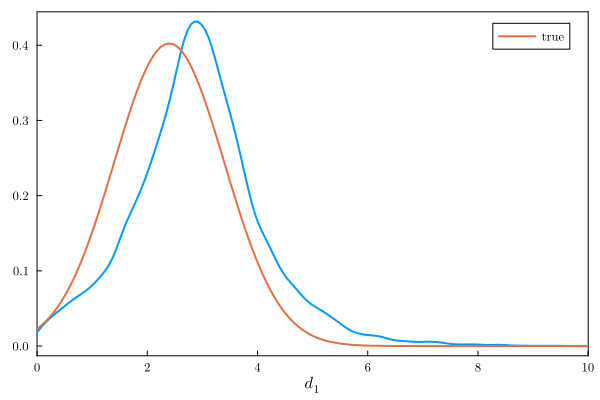
\includegraphics[scale=0.4]{d1_popu.png}
        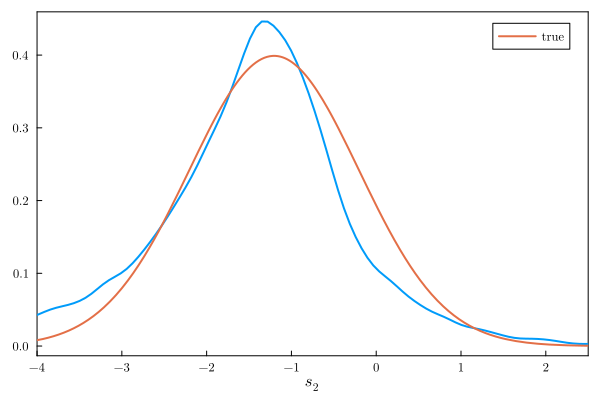
\includegraphics[scale=0.4]{s2_popu.png}
        \caption{Population distribution of the parameters of interest (true vs fitted)}
        \label{fig:pop_d1}
    \end{figure}

    \section{Validation of the multimodal hierarchical
        model}

    This model will be validated shortly.


\end{document} % This is the end of the document
